\chapter{Alternation} 
\label{chap:alts}

At present, we can write threads that try to send or receive on a
\emph{single} channel.  However, it's often useful to be able to try to send
or receive on either of two or more channels: the \emph{alternation}, or
\emph{alt}, construct does that for us.
%
We will start by describing the basic syntax of alternation, and then use it
in examples.

%%%%%

We start by describing how a thread can try to receive from any one of several
different in-ports.  The construct
%
\begin{scala}
  alt( 
    in£$_1$£ =?=> {f£$_1$£}
    | ...
    | in£$_n$£ =?=> {f£$_n$£}
  )
\end{scala}
%
waits until one of the in-ports \SCALA{in}$_1$, \ldots, \SCALA{in}$_n$
is ready to communicate, reads a value~$v$ from the port, and applies the
relevant function |f|$_i$ to~$v$.  If |in|$_i$ is an in-port passing data
of type~|A|, then $\sm f_i$ must be a function that takes an argument of
type~|A|. 

Here's a very simple example.  (The notation |x => c| represents a function
that, given argument~|x|, performs~|c|.)
%
\begin{scala}
  alt(
    c1 =?=> { x => println(s"$x received on c1") }
    | c2 =?=> { x => println(s"$x received on c2") }
  )
\end{scala}

%%%%%

The following thread repeatedly inputs from one of two input ports, tags the
value input, and outputs it.
%
\begin{mysamepage}
%  def tagger[T](l: ??[T], r: ??[T], out: !![(Int, T)]) = thread{
\begin{scala}
  repeat{
    alt ( l =?=> { x => out!(0, x) }
        | r =?=> { x => out!(1, x) }
    )
  }
\end{scala}
\end{mysamepage}
%
Exercise: design a corresponding de-tagger.  \framebox{??}

%%%%% \heading{Guards}

It's sometimes useful to specify that a particular in-port should be
considered only if some condition, or \emph{guard}, is true.  In the construct
%
\begin{scala}
  alt( guard£$_1$£ && in£$_1$£ =?=> {f£$_1$£}
     | ...
     | guard£$_n$£ && in£$_n$£ =?=> {f£$_n$£}
  )
\end{scala}
%
a communication on each |in|$_i$ is possible only if the corresponding
|guard|$_i$ is true.  Thus, \SCALA{in =?=> ...} is equivalent to \SCALA{true
  && in =?=> ...}.  Each guard is evaluated once, and should not have side
effects.

If a guard evaluates to true and the inport is open, we say that the
corresponding branch is \emph{feasible}.  If no branch is feasible, the alt
throws an |AltAbort| exception (a subclass of \SCALA{Stopped}): this
corresponds to the case where the alt will never be able to communicate.

If a branch is feasible and the inport is available for communication, then we
say that the branch is \emph{ready}.
%
The alt waits until a branch is ready, and receives from the inport.  If
several are ready, it chooses between them.  If all the branches become
infeasible (because of channels being closed), the alt throws an |AltAbort|
exception.

%%%%% \heading{\scalashape serve}

It is very common to use an \SCALA{alt} inside a \SCALA{repeat}.  Consider the
construct
%
\begin{scala}
  repeat{ 
    alt( g£$_1$£ && in£$_1$£ =?=> {f£$_1$£} | ... | g£$_n$£ && in£$_n$£ =?=> {f£$_n$£} ) 
  }
\end{scala}
%
Suppose no branch of the alt is feasible, that is, for every branch, either
the guard is false or the port is closed.  Then the alt will throw an
|AltAbort| exception, which the |repeat| will catch.  Thus the above construct
will repeatedly execute the alt until all branches become infeasible, at which
point it terminates cleanly.  

% (or one of the |f|$_i$ throws a |Stopped| exception).

Note that the above construct evaluates each guard expression~|g|$_i$ and each
port expression |in|$_i$ on each iteration.

%%%%% \heading{\scalashape serve}

The construct 
%
\begin{scala}
  serve( g£$_1$£ && in£$_1$£ =?=> {f£$_1$£} | ... | g£$_n$£ && in£$_n$£ =?=> {f£$_n$£} )
\end{scala}
%
is very similar to the previous |repeat{ alt(...) }| construct, but with two
differences.

One difference is that the earlier construct creates a new alternation object
(from a class |Alt|) on each iteration, whereas the |serve| creates a single
alternation object which is used repeatedly.

%%%%% \heading{Fairness}

The implementation of an alt tests whether its branches are ready in the order
given.  In the |repeat{alt(...)}| construct, a new alt object is created
for each iteration, so if the first branch is repeatedly ready, it will be
repeatedly selected, and the other branches will be starved.

By contrast, the |serve| aims to be fair.  It uses the same alt on each
iteration.  It remembers which branch was selected on the previous iteration,
and tests whether branches are ready starting from the following one (looping
round).
%
This means that if a particular branch is continuously ready, and the |serve|
performs enough iterations, then that branch will eventually be selected.  We
say that the |serve| is \emph{fair} to each branch.

%% Both the |serve| and the |repeat{alt(...)}| constructs evaluate each guard
%% expression~|g|$_i$ and each port expression |in|$_i$ on each iteration.

%%%%%

Here's the tagger again:
%
\begin{scala}
  serve( l =?=> { x => out!(0, x) } | r =?=> { x => out!(1, x) } )
\end{scala}
%
Note that this is fair to its two input ports: once one becomes ready, the
|serve| will receive from it after at most one communication on the other
port.
%
The |serve| loop terminates when either both |l| and~|r| are closed, or |out|
is closed. 

%%%%% \heading{About fairness}

Fairness crops up in a number of scenarios in concurrent programming.
%
A typical fairness property is that if a particular option is continually
logically possible, then it eventually happens.  Fairness for an alt
construct means that if a particular branch is continually ready, and the
alt performs enough iterations, then eventually that branch is selected.

Note that ``fair'' doesn't necessarily mean equal shares: a construct that
chooses option~$A$ 99\% of the time, and chooses option~$B$ 1\% of the time is
fair despite not giving equal shares.

Fairness is psychologically attractive: certainly, being fair to other people
in everyday life is a good thing.  However, it's not always appropriate in a
concurrent program.  In some scenarios, achieving fairness has a performance
overhead.  And sometimes fairness can be achieved only by a more complicated
program.  You should consider whether or not fairness is desirable.  Often you
can achieve higher throughput, and a simpler program, without fairness.
 % Introduction
\section{Example: The Dining Philosophers}

The Dining Philosophers problem is an example formulated by Edsger Dijkstra
to illustrate some of the problems that can arise in concurrent programming.  
It is presented in terms of interactions between people; but it is an analogy
for concurrent threads or processes sharing resources. 

Five philosophers spend most of their lives thinking; but sometimes they need
to eat.  They share a common dining room, which has a circular table with five
chairs around it, a plate in front of each chair, and a big bowl of spaghetti
in the middle.  There are five forks, placed between the five plates at the
table; a philosopher needs two forks in order to eat the spaghetti. 

When a philosopher gets hungry, they sit down.  They pick up the fork to their
left as soon as it's available (they might need to wait for their left-hand
neighbour to finish with the fork).  Then they pick up the fork to their right
as soon as it's available.  Once the philosopher has two forks, they serve
themself and spend some time eating.  The philosopher then puts the forks
down, leaves the table, and does some more thinking.

However, there is a problem with this protocol.  If all five philosophers get
hungry at about the same time and pick up their left fork, then they are
unable to obtain their right fork, and so all starve!  Of course, real
philosophers---being smart people---would soon solve the problem.  But if we
think of this as an analogy for concurrent threads, the program would not.

We will build a simulation of the Dining Philosophers example.  We 
simulate each philosopher and each fork by a thread.  The first part of the
simulation is in Figure~\ref{fig:dining-phils-1}.  We denote the number of
philosophers by~|N|; this allows us to easily vary the number. 

%%%%%%%%%%

\begin{figure}
\begin{scala}
/** Simulation of the Dining Philosophers example. */
object Phils{
  val N = 5 // Number of philosophers.

  // Simulate basic actions.
  def eat() = Thread.sleep(500)
  def think() = Thread.sleep(scala.util.Random.nextInt(900))
  def pause() = Thread.sleep(500)

  type Cmd = Boolean; val Pick = true; val Drop = false
 
  /** A single philosopher. */
  def phil(me: Int, left: !![Cmd], right: !![Cmd]) = thread(s"Phil $me"){
    repeat{
      think()
      println(s"$me sits"); pause()
      left!Pick; println(s"$me picks up left fork"); pause()
      right!Pick; println(s"$me picks up right fork"); pause()
      println(s"$me eats"); eat()
      left!Drop; pause(); right!Drop; pause()
      println(s"$me leaves")
    }
  } 

  /** A single fork. */
  def fork(me: Int, left: ??[Cmd], right: ??[Cmd]) = thread(s"Fork $me"){
    serve(
      left =?=> {x => assert(x == Pick); val y = left?(); assert(y == Drop)}
      |
      right =?=> {x => assert(x == Pick); val y = right?(); assert(y == Drop)}
    )
  } 
  ...
}
\end{scala}
\caption{The Dining Philosophers example (part 1).}
\label{fig:dining-phils-1}
\end{figure}

%%%%%%%%%%

We simulate the actions of eating and thinking, and a pause between other
actions, by having the thread sleep for a short period (the library method
|Thread.sleep(t)| suspends the current thread for |t|\,ms).

We simulate the picking up and putting down of forks by the philosopher
thread sending a suitable value, |Pick| or |Drop|, respectively, to the fork
thread.  We denote the type of these values as~|Cmd|.  We choose to represent
the values as |Boolean|s.

The philosopher thread |phil| is parameterised by the philosopher's identity,
and out-ports on which it can send messages to its left- and right-hand forks.
The definition is then a straightforward translation of the earlier informal
description, sending |Pick| and~|Drop| messages to simulate the picking up and
dropping of the fork.  The code prints messages to the screen describing the
philosopher's actions.

The fork thread is parameterised by the fork's identity, and in-ports on which
it can receive messages from its left- and right-hand philosopher.  The fork
should initially be willing to receive a message on \emph{either} of its
in-ports.  Modelling this requires an alternation, in this case via a |serve|
construct.  The value it receives should be a |Pick|.  It then waits to
receive a second message on the same in-port, which should be a |Drop|.  The
|assert| statements check the correct messages are received.  Using assertions
like this is good practice.  If nothing else, it acts as good documentation.
But such assertions can also help to catch mistakes.  (I have found lots of
mistakes in my own code by including assertions like these.  If I had omitted
those assertions, it would probably have led to errors arising later in the
program, but it would have been much harder to identify the cause of the
problem.)

We connect the philosophers and forks together as depicted in the top half of
Figure~\ref{fig:dining-philosophers-2}, with the corresponding code in the
bottom half of the figure.  We use two arrays of channels, indexed by the
identities of the philosophers: channel |philToLeftFork(i)| is from |phil(i)|
to |fork(i)|; and channel |philToRightFork(i)| is from |phil(i)| to
|fork(|$(\sm i-1) \bmod \sm N$|)|.  It is easy to get confused about the
indexing of arrays of channels in cases like this: I recommend drawing a
picture and writing a clear comment.  

%%%%%%%%%%

\begin{figure}
\begin{center}
\def\r{4.07}
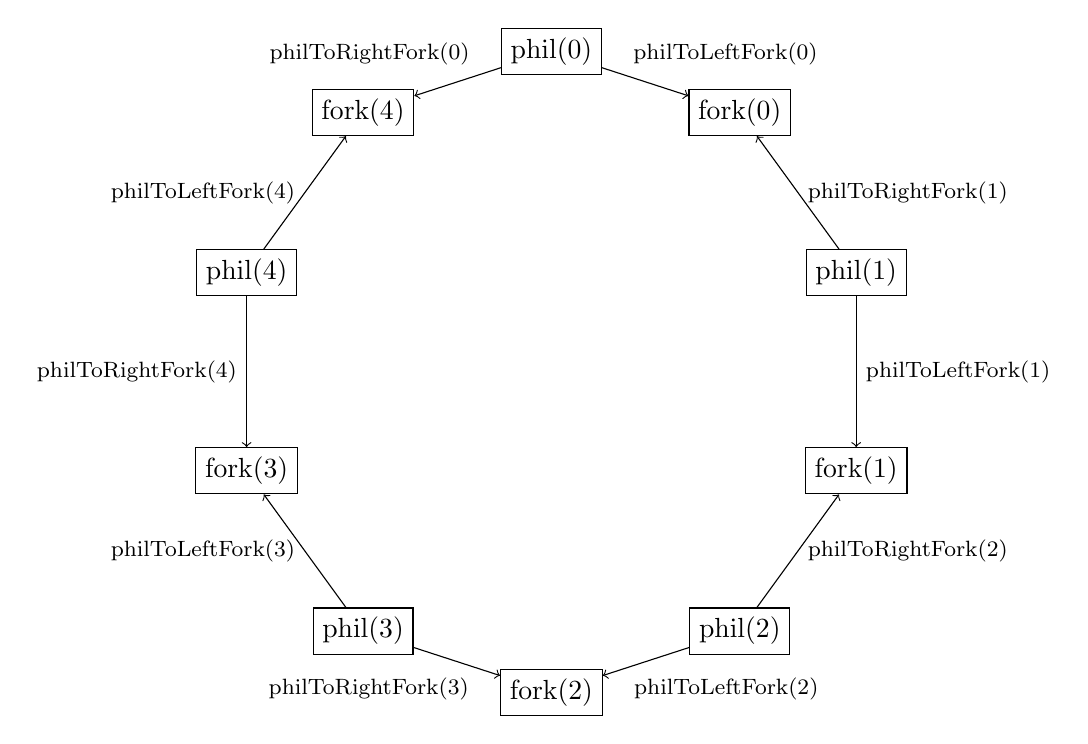
\begin{tikzpicture}
\foreach \i in {0,...,4} 
  \draw (90-72*\i: \r) node[draw] (phil\i) {\scalashape phil(\i)}; 
\foreach \i in {0,...,4} 
  \draw (54-72*\i: \r) node[draw] (fork\i) {\scalashape fork(\i)}; 
%
\draw[->] (phil0) -- node[above right, near start] 
  {\scalashape\footnotesize philToLeftFork(0)} (fork0);
\draw[->] (phil1) -- node[right] 
  {\scalashape\footnotesize philToLeftFork(1)} (fork1);
\draw[->] (phil2) -- node[below right, near end] 
  {\scalashape\footnotesize philToLeftFork(2)} (fork2);
\draw[->] (phil3) -- node[left] 
  {\scalashape\footnotesize philToLeftFork(3)\ } (fork3);
\draw[->] (phil4) -- node[left] 
  {\scalashape\footnotesize philToLeftFork(4)\ } (fork4);
%
\draw[->] (phil0) -- node[above left, near start]
  {\scalashape\footnotesize philToRightFork(0)} (fork4);
\draw[->] (phil1) -- node[right]
  {\scalashape\footnotesize philToRightFork(1)} (fork0);
\draw[->] (phil2) -- node[right]
  {\scalashape\footnotesize philToRightFork(2)} (fork1);
\draw[->] (phil3) -- node[below left, near end]
  {\scalashape\footnotesize philToRightFork(3)} (fork2);
\draw[->] (phil4) -- node[left]
  {\scalashape\footnotesize philToRightFork(4)} (fork3);
\end{tikzpicture}
\end{center}

%%%%%

\begin{scala}
  /** The complete system. */ 
  def system = {
    val philToLeftFork, philToRightFork = Array.fill(N)(new SyncChan[Cmd])
    // £philToLeftFork(i)£ is from £phil(i)£ to £fork(i)£;
    // £philToRightFork(i)£ is from £phil(i)£ to £fork($(\sm i-1) \bmod \sm N$)£.
    val allPhils = || ( 
      for (i <- 0 until N) yield phil(i, philToLeftFork(i), philToRightFork(i))
    )
    val allForks = || ( 
      for (i <- 0 until N) yield
        fork(i, philToRightFork((i+1)%N), philToLeftFork(i))
    )
    allPhils || allForks
  }

  /** Run the system. */
  def main(args : Array[String]) = run(system)
\end{scala}
\caption{The Dining Philosophers example (part 2).}
\label{fig:dining-philosophers-2}
\end{figure}

%%%%%%%%%%%

It is important that we use \emph{synchronous} channels: we need each
philosopher and fork to synchronise on relevant actions. 

\begin{instruction}
Study the details of the implementation.
\end{instruction}

When we run the system, sometimes it deadlocks almost immediately.  A~typical
deadlocking trace is:
%
\begin{scala}
1 sits,  0 sits,  4 sits,  2 sits,  1 picks up left fork, 3 sits,  0 picks up left fork,  
4 picks up left fork, 2 picks up left fork,  3 picks up left fork
\end{scala}
%
Each philosopher sits down and picks up their left fork (in some order).  At
this point, each philosopher is trying to pick up its right fork, i.e.~to send
a |Pick| message on its |right| channel; however, the corresponding fork is
not willing to receive that message.  This means that the system is
deadlocked.

Recall that typing \texttt{Ctrl}+$\backslash$ (control and backslash) produces
a thread dump.  This gives the line number in the code where each thread is
stuck, so can help to understand the deadlock.

However, sometimes when we run the system, it runs for a very long time
without deadlocking.  In fact, I chose the delays in the simulations of the
basic actions so that the system deadlocks about half the time.  Different
choices for these delays would have caused the system to deadlock on nearly
every run, or hardly ever.  In some ways, the latter situation is worse: it is
likely that the potential deadlock would not be found by routine testing, but
that it would occur only when the system is deployed.

%%%%%%%%%%%%%%%%%%%%%%%%%%%%%%%%%%%%%%%%%%%%%%%%%%%%%%%%%%%%%%%%%

\section{Logging and Debugging}

In the above simulation, we used |println| statements so that we could
understand what happened.  However, this style is often not convenient when
tracking down bugs.  Normally, a better way to is to use logging.

The SCL class |Log| provides log objects.
%
A new log storing events of type~|A|, suitable for |p| threads,
can be defined by
\begin{scala}
  val log = new Log[A](p)
\end{scala}
%
This provides operations
%
\begin{itemize}
\item |def add(me: Int, x: A)|, which adds |x| to the log, performed by
  thread~|me|, where $\sm{me} \in \interval{0}{\sm p}$;

\item |def get: Array[A]|, which gets the contents of the log;

\item |def toFile(fname: String = "/tmp/logFile")|, which writes the contents
  of the log to the file~|fname| (with a default of \texttt{/tmp/logFile}).
\end{itemize}

The code in Figure~\ref{fig:dining-phils-log} shows how we can use logging in
the dining philosophers example.  (I have arranged for philosopher~|0| to
print a dot on each iteration, so we can tell whether the system is making
progress.)

%%%%%

\begin{figure}
\begin{scala}
  val log = new Log[String](N)
 
  def phil(me: Int, left: !![Cmd], right: !![Cmd]) = thread(s"Phil $me"){
    repeat{
      think()
      log.add(me, s"$me sits"); pause()
      left!Pick; log.add(me, s"$me picks up left fork"); pause()
      right!Pick; log.add(me, s"$me picks up right fork"); pause()
      log.add(me, s"$me eats"); eat()
      left!Drop; pause(); right!Drop; pause()
      log.add(me, s"$me leaves")
      if(me == 0) print(".")
    }
  }
\end{scala}
\caption{Using a {\scalashape Log} object.}
\label{fig:dining-phils-log}
\end{figure}

%%%%%

In many scenarios, when the system terminates, we can either write the log to
a file, or analyse the log using some code.  However, this won't work when the
system deadlocks.  Instead, we need to insert a hook that will arrange for the
log to write itself to a file when the user interrupts the program.  This can
be done with the |writeToFileOnShutdown| method:
%
\begin{scala}
  def main(args: Array[String]) = {
    log.writeToFileOnShutdown("philsLog.txt"); run(system)
  }
\end{scala}

Logging is a general technique that can help with debugging.  However, there
is a wrinkle concerning its usage.
%
Internally, each thread uses its own thread-local log, to avoid race
conditions, and for efficiency.  This is why the |log| operation takes the
thread's identity as a parameter: different threads should use different
identities, in the relevant range.  Each logged value is stored in the
relevant thread-local log, together with a timestamp (more precisely, the
time elapsed since the |Log| object was created, to avoid problems with
timestamp wrap-around).
%
The |get| operation merges the thread-local logs according to
timestamps.

Using timestamps in this way assumes that the clocks are loosely synchronised
across cores, and that the granularity of the clocks is sufficiently fine, so
that if one |add| event logically happens before another (i.e.~according to
the~$\prec$ relation), the former receives a strictly smaller timestamp.

The above assumption seems to be sound in Linux, but not in Windows.  If you
must use Windows, the class |SharedLog| provides the same interface.  However,
it will give worse performance.  Further, it might affect the likelihood of
detecting bugs: I have experienced bugs that would appear when no logging was
performed, or when the timestamp-based log was used; but logging with
something equivalent to |SharedLog| affected the speed of threads sufficiently
that the bug no longer appeared in a reasonable time!


 % Dining Philosophers, logging.
\section{Alts with out-ports}

So far, we have only seen alts that provide a choice between in-ports.
However, it is also possible to use an out-port in an alt, using the following
syntax:%
%
\begin{scala}
  bool && out =!=> { expression }
\end{scala}
%
If the (optional) boolean guard |bool| is true, when the out-port |out| is
ready for communication, the |expression| is evaluated and the result sent.

Sometimes it's necessary to do something \emph{after} the value has been sent,
using a continuation, with the following syntax.
%
\begin{scala}
   bool && outport =!=> { expression } ==> { command }
\end{scala}

For example, here's another definition for the |tee| function, which produces
a thread that inputs on one in-port, and outputs on two out-ports, in either
order. 
%
\begin{mysamepage}
\begin{scala}
def tee[T](in: ??[T], out1: !![T], out2: !![T]) = thread{
  repeat{ 
    val v = in?()
    alt( out1 =!=> { v } ==> { out2!v }
       | out2 =!=> { v } ==> { out1!v }
    )
  }
}
\end{scala}
%
This sends~|v| on whichever out-port is ready first, and then sends~|v| on the
other out-port.
\end{mysamepage}

%%%%%% A two-place buffer

Inports and outports can be mixed within an \SCALA{alt}.
%
The following code copies data from |in| to |out|, and can hold up to two
pieces of data at a time: it is a two-place buffer. 
%
\begin{scala}  
  /** Two place buffer. */
  def buff2[T](in: ??[T], out: !![T]): Unit = {
    val x = in?(); buff2A(in, out, x)
  }
  /** Two place buffer holding £x£. */
  def buff2A[T](in: ??[T], out: !![T], x: T): Unit = {
    alt(
      out =!=> { x } ==> { buff2(in, out) }
      | in =?=> { y => out!x; buff2A(in, out, y) }
    )
  }  
\end{scala}
%
Note how when it is holding a value~|x|, it can either output~|x|, or input a
new value~|y|, at which point it is full so must output~|x|, after which it is
just holding~|y|.


Here's an alternative definition.  The variable \SCALA{empty} records whether
the buffer is empty.  When $\sm{empty} = \sm{false}$,\, \SCALA{x} stores the
next value to be output.
%
\begin{scala}
  def buff2Alt[T](in: ??[T], out: !![T]) = {
    var x: T = null.asInstanceOf[T]  // Contents, possibly invalid.
    var empty = true // Is the buffer empty?
    serve(
      !empty && out =!=> { empty = true; x }
      | empty && in =?=> { v => x = v; empty = false }
      | !empty && in =?=> { v => out!x; x = v }
    )
  }
\end{scala}
%
In the first branch, the code \SCALA{\{ empty = true; x \}} is an expression
whose value is~|x|, but which has the side effect of setting |empty| to |true|. 
The last two branches could be merged, and an \SCALA{if} statement used. 
%
\begin{scala}
    | in =?=> { v => if(empty){ x = v; empty = false } else { out!x; x = v } }
\end{scala}


\framebox{Quicksort}
 % Avoiding deadlocks, With outports
\section{Example: Bag of Tasks with Replacement}
\label{sec:quicksort-bag}

In Chapter~\ref{chap:trapezium} we say the bag-of-tasks pattern, where workers
repeatedly obtain a task, and perform it.  We now consider a variant, where
workers can return subtasks to the bag.  Thus, if a worker obtains a
task~$t$, it will perform some work itself, and (maybe) return some subtasks to
the bag; these together must equate to completing~$t$.

In particular, we will use the bag-of-tasks with replacement pattern to
produce a concurrent implementation of the Quicksort sorting algorithm.
Figure~\ref{fig:quicksort-seq} gives a sequential implementation of the
algorithm.  

%%%%%

\begin{figure}
\begin{scala}
/** Trait implemented by different implementations of Quicksort. */
trait QuicksortT{
  protected val a: Array[Int]

  /** Partition £$\sm a\interval{\sm l}{\sm r}$£, returning the index of the pivot. */
  protected def partition(l: Int, r: Int): Int = {
    assert(r-l > 1)
    val x = a(l); var i = l+1; var j = r
    while(i < j){
      while(i < j && a(i) <= x) i += 1
      while(i < j && a(j-1) > x) j -= 1
      if(i < j){ // £$\sm a(\sm i) > \sm x \land \sm a(j\sm -1) \le \sm x$£, so swap.
        val t = a(i); a(i) = a(j-1); a(j-1) = t 
      }
    }
    // Swap pivot into position £i-1£, and return that index.
    a(l) = a(i-1); a(i-1) = x; i-1
  }
}

/** Sequential implementation of Quicksort. */
class Quicksort(protected val a: Array[Int]) extends QuicksortT{
  /** Sort a. */
  def sort() = qsort(0, a.length)

  /** Sort the segment a[l..r). */
  private def qsort(l: Int, r: Int): Unit =
    if(r-l > 1){ val m = partition(l, r); qsort(l,m); qsort(m+1,r) }
}
\end{scala}
\caption{A sequential implementation of Quicksort.}
\label{fig:quicksort-seq}
\end{figure}

%%%%%

The function |partition(l, r)| partitions the non-empty segment $\sm
a\interval{\sm l}{\sm r}$.  It picks some element~|x| from the segment, and
permutes the elements of the segment so that it looks like this:
\[\mstyle
\begin{array}{rllclcll}
   & 0 & \ms{l} & & \ms{k} &  & \ms{r} & \ms{N} \\ \cline{2-7}
\multicolumn{1}{r\|}{\ms{a}:\;} & \qquad\qquad & 
  \multicolumn{2}{\|c\|}{\quad \le \ms{x} \quad} & 
  \multicolumn{1}{c\|}{\ms{x}} &
  \multicolumn{1}{c\|}{\quad > \ms{x} \quad} &
  \multicolumn{1}{c\|}{\qquad\qquad}  \\ \cline{2-7}
\end{array}
\]
More precisely, it returns an index~|k| such that
\[\mstyle
\sm a\interval{\sm l}{\sm k} \le \sm a(\sm k) < 
  \sm a\interval{\sm k+1}{\sm r} 
\land \sm l \le \sm k < \sm r.
\]

The implementation of~|partition| chooses the first element |a(l)| as the
pivot~|x|.  The main loop keeps |x| in position~|l|; it is swapped into the
correct position only at the end.  The loop maintains the invariant
\[\mstyle
\sm a\interval{\sm l+1}{\sm i} \le \sm x = \sm a(\sm l) < 
  \sm a\interval{\sm j}{\sm r} 
\land \sm l < \sm i \le \sm j \le \sm r,
\]
which we can picture as follows.
\[\mstyle
\begin{array}{rllclcllll}
   & 0 & \ms{l} & \ms{l+1} & & \ms{i} &  & \ms{j} & \ms{r} & \ms{N} 
\\ \cline{2-9}
\multicolumn{1}{r\|}{\ms{a}:\;} & \qquad\qquad & 
  \multicolumn{1}{\|c\|}{\ms{x}} &
  \multicolumn{2}{c\|}{\quad \le \ms{x} \quad} & 
  \multicolumn{2}{c\|}{\quad?\quad} &
  \multicolumn{1}{c\|}{\quad > \ms{x} \quad} &
  \multicolumn{1}{c\|}{\qquad\qquad}  \\ \cline{2-9}
\end{array}
\]
(We include the |partition| function in the |QuicksortT| trait, to avoid
repeating code; each of our implementations will extend this trait.)

Most of the work is done by the function |qsort(l, r)|, which sorts the
segment $\sm a\interval{\sm l}{\sm r}$.  If the interval contains at most one
element, then it is already sorted.  Otherwise, the function calls partition,
and then recursively sorts the two subintervals.  The main |sort| function
calls |qsort| on the whole array.

\begin{instruction}
Make sure you understand the code in Figure~\ref{fig:quicksort-seq}.
\end{instruction}

%%%%%%%%%%

\subsection{Basic Concurrent Implementation}

We will create two concurrent implementations of the Quicksort algorithm, each
based upon the bag-of-tasks pattern.  The implementation in this section will
be straightforward, but rather inefficient; we will produce a more efficient
implementation in the next section.

Each task will be represented by a pair |(l,r)|, and will represent the task
of sorting the interval $\sm a\interval{\sm l}{\sm r}$, rather like the
earlier function |qsort(l, r)|.  We define
\begin{scala}
  type Task = (Int, Int)
\end{scala}
%
If the interval $\sm a\interval{\sm l}{\sm r}$ contains at least two elements,
the worker will partition it, and then return to the bag two subtasks
corresponding to the two subintervals.  Once these subtasks are completed, the
interval $\sm a\interval{\sm l}{\sm r}$ will be sorted.

We need to think about termination.  The whole array will be sorted when the
bag is holding no tasks, and no worker is working on a task.  Thus the server
implementing the bag needs to keep track of how many workers are working on
tasks.  It can increment this count when it issues a task, and can decrement
the count when a worker returns two subtasks.  However, when a worker receives
a task containing at most one element, the worker will return no subtasks, so
it needs a different way to indicate that the task is complete.

We encapsulate the bag of tasks in an object~|Bag|, as in
Figure~\ref{fig:quicksort-bag-1}.   The operation |get| allows a worker to get
a task.  The operation |add| allows a worker to return two subtasks to the
bag.  The operation |done| allows a worker to signal that it has completed a
task (without returning subtasks).  

%%%%%%%%%%

\begin{figure}
\begin{scala}
  object Bag{
    private val getC = new SyncChan[Task]
    private val addC = new SyncChan[(Task,Task)]
    private val doneC = new SyncChan[Unit]

    /** Get a £Task£. */
    def get(): Task = getC?()

    /** Add £Task£s £t1£ and £t2£ to the bag. */  
    def add(t1: Task, t2: Task): Unit = addC!(t1,t2)

    /** Indicate that the current thread has completed its last £Task£. */
    def done(): Unit = doneC!()

    private def server = thread("server"){
      val queue = new scala.collection.mutable.Queue[Task]
      queue.enqueue((0, a.length)); var busyWorkers = 0
      serve(
        queue.nonEmpty && getC =!=> { busyWorkers += 1; queue.dequeue() }
        | busyWorkers > 0 && addC =?=> { case (t1,t2) => 
            queue.enqueue(t1); queue.enqueue(t2); busyWorkers -= 1 }
        | busyWorkers > 0 && doneC =?=> { _ => busyWorkers -= 1 }
      )
      assert(queue.isEmpty && busyWorkers == 0)
      getC.endOfStream()
    }

    fork(server)
  } 
\end{scala}
\caption{The bag of tasks in the basic concurrent implementation of Quicksort.}
\label{fig:quicksort-bag-1}
\end{figure}

%%%%%%%%%%

The |Bag| object encapsulates a server thread.  Each operation is implemented
by a single communication between the worker and the server.  Note, in
particular, that the |add| operation sends both subtasks in a single message,
rather than two separate messages: this roughly halves the cost of the
operation. 

The server itself stores the pending tasks in a queue (although we could have
used a different collection class, such as a stack).  It also uses a variable
|busyWorkers| to record the number of workers currently working on a task.
Most of the implementation is then fairly straightforward.  The main |serve|
loop terminates when all the guards are false, namely when the queue is empty
and $\sm{busyWorkers} = 0$: this is the termination condition we identified
earlier.  Note in particular how that second and third branches each has a
guard |busyWorkers > 0| in order to achieve this termination condition: and we
should certainly expect this condition to hold whenever a worker tries to send
on |addC| or |doneC|.  When the |serve| loop terminates the server performs
|endOfStream| on the |getC| channel, to signal to the workers that there are
no more tasks to complete.
%
\begin{instruction}
Make sure you understand the implementation of |Bag|.
\end{instruction}

The main implementation is in Figure~\ref{fig:quicksort-bag-of-tasks-1}.  Each
worker repeatedly gets a task from the bag.  If the task contains more than
one element, the worker partitions it, and returns the two subtasks to the
bag.  Otherwise, it informs the bag that the task is complete via the |done|
operation.  The worker terminates when the |get| operation throws a |Stopped|
exception, which corresponds to the termination condition described earlier.
The main |sort| function simply runs |numWorkers| workers.  

%%%%%%%%%%

\begin{figure}
\begin{scala}
/** Basic concurrent implementation. */
class ConcurrentQuicksort1(protected val a: Array[Int], numWorkers: Int)
    extends QuicksortT{
  type Task = (Int, Int)

  object Bag{
    £\ldots£ // as in Figure £\ref{fig:quicksort-bag-1}£.
  }

  /** A single worker. */
  private def worker = thread("worker"){
    repeat{
      val (l,r) = Bag.get()
      if(r-l > 1){ val m = partition(l, r); Bag.add((l,m), (m+1,r)) }
      else Bag.done()
    }
  }

  /** Sort £a£. */
  def sort() = run(|| (for(i <- 0 until numWorkers) yield worker))
}
\end{scala}
\caption{The basic implementation of Quicksort using a bag of tasks.}
\label{fig:quicksort-bag-of-tasks-1}
\end{figure}

%%%%%

The implementation can be tested by checking that it produces the same results
as the sequential implementation from Figure~\ref{fig:quicksort-seq}.  We can
create a random array of |Int|s, clone it, run the two algorithms on the two
copies, and check the two results contain the same elements.  This can be
repeated many times.

Unfortunately, this implementation performs poorly.  On an array containing a
million values, it is about 100 times slower than the sequential algorithm.
The main reason for this is that there are simply too many messages sent over
channels, and this creates a very large overhead.  For example, consider a
subtask containing just two elements; this will lead to one message issuing
that task, two messages returning the two subtasks, two messages issuing those
subtasks, and two messages indicating that those subtasks are done, for a
total of seven messages.  The following subsection seeks to improve this.


%%%%%%%%%%%%%%%%%%%%%%%%%%%%%%%%%%%%%%%%%%%%%%%%%%%%%%%

\subsection{Improved Concurrent Implementation} 

We can improve the implementation in several ways.
%
\begin{enumerate}
\item \label{obs:quicksort-1}
  Rather than returning two subtasks to the bag, a worker could return
  just one, and complete the second task itself.  This means that we save a
  message in each such case.

\item There is no point in returning subtasks to the bag if they contain at
  most one element, since those subtasks require no additional work.  This
  greatly reduces the number of messages corresponding to such subtasks.  We
  call subtasks with at most one element \emph{trivial}. 

\item\label{obs:quicksort-3} If a worker receives a task that is fairly small,
  it is more efficient for the worker to complete the whole task itself, using
  the sequential algorithm, rather than creating new subtasks.
\end{enumerate}

Figure~\ref{fig:quicksort-bag-2} gives a new definition of the bag of tasks.
The only change corresponds to observation~\ref{obs:quicksort-1} above.  Now
the |add| operation returns a single task; the server does not decrement
|busyWorkers| as a result, as the relevant worker is still working on the
other subtask. 

%%%%%%%%%%%%%%%%

\begin{figure}
\begin{scala}
  object Bag{
    private val getC = new SyncChan[Task]
    private val addC = new SyncChan[Task]
    private val doneC = new SyncChan[Unit]

    def get(): Task = getC?()

    def add(t: Task): Unit = addC!t

    def done(): Unit = doneC!()

    private def server = thread("server"){
      val queue = new scala.collection.mutable.Queue[Task]
      queue.enqueue((0, a.length)); var busyWorkers = 0
      serve(
        queue.nonEmpty && getC =!=> { busyWorkers += 1; queue.dequeue() }
        | busyWorkers > 0 && addC =?=> { t => queue.enqueue(t) }
        | busyWorkers > 0 && doneC =?=> { _ => busyWorkers -= 1 }
      )
      assert(queue.isEmpty && busyWorkers == 0)
      getC.endOfStream()
    }

    fork(server)
  } 
\end{scala}
\caption{The bag of tasks in the improved concurrent algorithm.}
\label{fig:quicksort-bag-2}
\end{figure}

%%%%%

The main implementation is in Figure~\ref{fig:quicksort-bag-of-tasks-2}.  For
the purposes of observation~\ref{obs:quicksort-3}, above, we consider a task
to be small if it contains fewer than |Limit| elements, where |Limit| is
defined as the minimum of $20,000$ and $\sm{a.size} / (10 \times
\sm{numWorkers})$.  My informal experiments suggested that for tasks smaller
than about $20,000$, it is faster for the worker to complete the whole task
itself than to create subtasks.  The latter term means that for very large
arrays, each worker can sort larger segments sequentially; the value ensures
that on average each worker sorts slightly fewer than ten segments
sequentially, which seems enough to give reasonable load balancing.  If
out-and-out performance was important, we could run further experiments to
tune these figures.

%%%%%

\begin{figure}
\begin{scala}
class ConcurrentQuicksort2(protected val a: Array[Int], numWorkers: Int)
    extends QuicksortT{
  type Task = (Int, Int)

  object Bag{
    £\ldots£ // As in Figure £\ref{fig:quicksort-bag-2}£.
  }

  /** Upper limit on the size of tasks sorted sequentially. */
  val Limit = 20_000 max (a.size / (10*numWorkers))

  /** Sequential implementation. */
  private def qsort(l: Int, r: Int): Unit =
    if(r-l > 1){ val m = partition(l, r); qsort(l,m); qsort(m+1,r) }

  /** A single worker. */
  private def worker = thread("worker"){
    var l = -1; var r = -1
    repeat{
      if(l == r){ val task = Bag.get(); l = task._1; r = task._2; assert(r-l > 1)}
      }  
      if(r-l < Limit){ qsort(l,r); r = l; Bag.done() }
      else{
        val m = partition(l, r)
        if(m-l > 1){ // Continue with £(l,m)£.
          if(r-(m+1) > 1) Bag.add((m+1,r))
          r = m
        }
        else if(r-(m+1) > 1) l = m+1 // Continue with £(m+1,r)£.
        else{ r = l; Bag.done() } // This segment finished.
      }
    }
  }

  def sort() = if(a.size > 1) run(|| (for(i <- 0 until numWorkers) yield worker))
}
\end{scala}
\caption{The improved implementation of Quicksort using a bag of tasks.}
\label{fig:quicksort-bag-of-tasks-2}
\end{figure}

%%%%%

The worker maintains two variables |l| and~|r|, with $\sm l \le \sm r$.  If
$\sm l < \sm r$, then this worker is still responsible for the segment $\sm
a\interval{\sm l}{\sm r}$.  But if $\sm l = \sm r$, the worker has no current
task.  In the latter case, the worker obtains a new task from the bag, and
unpacks it.  In either case, if the task is smaller than |Limit|, it sorts it
sequentially, sets~|r| to~|l| to record that the task is done, and signals
that fact to the bag.  Otherwise, it partitions the segment, to obtain a pivot
index~|m|.  If the subsegment $\sm a\interval{\sm l}{\sm m}$ is not trivial,
it continues with that subsegment, and returns the task for the other
subsegment to the bag if it is not trivial.  Otherwise, if the subsegment $\sm
a\interval{\sm m+1}{\sm r}$ is not trivial, it continues with that subsegment.
Otherwise, the task is complete, so it updates |r| to record that, and signals
that fact to the bag.

%This implementation is far faster than the previous concurrent implementation.
For arrays of size 1,000,000, using eight workers, this implementation is
slightly faster than the sequential implementation, so about 100 times
faster than the previous concurrent implementation.  For arrays of size
10,000,000, it is about four times faster than the sequential
implementation; and for arrays of size 100,000,000, it is about five times
faster.
 % quicksort bag of tasks example.

%%%%%%%%%%%%%%%%%%%%%%%%%%%%%%%%%%%%%%%%%%%%%%%%%%%%%%%%%%%%

\section{Summary}

In this chapter, we have studied \emph{alternation} constructs, whereby a
thread can try to communicate on any one of several different ports.  We
have seen several examples using alternation.  In particular, we saw how it
could be used to implement a bag of tasks with replacement. 

There is quite a lot of syntax involved with alternations: |alt| and |serve|;
in-port branches and out-port branches; guards; and indexed alternations.  You
should make sure you are familiar with the syntax.

There are two restrictions on the use of alternations: a port may not be
simultaneously feasible in two alternations; and both ports of a channel may
not be simultaneously feasible in alternations.  (Each restriction represents
a design choice, to make the implementation of alternation simpler and more
efficient.)

Along the way, we discussed how to use logging to help with debugging; later
we will use similar techniques for testing.  We also discussed how to identify
possible deadlocks as cycles of waiting, and how to avoid them.

As a caveat, you should note that alternations are fairly heavyweight
constructs.  Under the bonnet, the implementation has to do quite a lot of
work to identify whether any of its ports is ready for communication.  Don't
use an alternation unless there is a good reason to do so, i.e.,~you really
need a thread to be able to communicate on either of two channels.  Sometimes
it's easier and more efficient to force communications to happen in a
particular order, rather than allowing multiple different orders.

Sometimes a shared channel can produce the same effect as an \SCALA{alt}.  For
example, we could construct a variant of the dining philosophers where each
philosopher has channels \SCALA{pick} and \SCALA{drop} for each of its forks,
and where each fork has single \SCALA{pick} and \SCALA{drop} channels, on
which it can receive messages from either of the adjacent philosophers:
%
\begin{scala}
  def Fork(me: Int, pick: ??[Unit], drop: ??[Unit]) = thread("Fork"+me){
    repeat{ pick?(); drop?() }
  }
\end{scala}
%
%% Note that the \SCALA{pick} communication could be from either neighbouring
%% philosopher, so these need to be |ManyOne| channels.
Note that we need separate |pick| and |drop| channels, so that when one of the
philosophers is holding the fork, the other cannot pick it up.  However, such
a technique isn't always applicable. 

%%%%%%%%%%%%%%%%%%%%%%%%%%%%%%%%%%%%%%%%%%%%%%%%%%%%%%%

\section*{Exercises}
 
\begin{questionS}
Design a \emph{change machine}  with signature:
%
\begin{scala}
  def ChangeMachine(
      inPound: ??[Unit], out5p: !![Unit], out10p: !![Unit], out20p: !![Unit]
  ) = thread{...}
\end{scala}
%
where communications on the channels correspond to the insertion of \pounds 1,
and the output of a 5p, 10p or 20p piece, respectively.  It should be willing
to accept \SCALA{inPound} whenever it had a zero balance.  It should offer
the environment the choice between how it wants the change, subject to the
condition that it should not output coins of more value than it has received. 
\end{questionS}

%%%%%

\begin{answerS}
My solution is below.  Each branch needs a suitable guard. 
%
\begin{scala}  
  def ChangeMachine(
      inPound: ?[Unit], out5p: ![Unit], out10p: ![Unit], out20p: ![Unit]
  ) = thread{
    var credit = 0 // Credit in pence.
    serve(
      credit == 0 && inPound =?=> { () => credit += 100 }
      | credit >= 5 && out5p =!=> { credit -= 5; () }
      | credit >= 10 && out10p =!=> { credit -= 10; () }
      | credit >= 20 && out20p =!=> { credit -= 20; () }
    )
  }
\end{scala}
\end{answerS}
 % Change machine 

\begin{question}
Implement an unbounded buffer:
%
\begin{scala}
def buff[T](in: ??[T], out: !![T]) = thread{ ... }
\end{scala}
%
The buffer should always be willing to input on \SCALA{in}; it should output
data on \SCALA{out} in the order in which they were received, and should be
willing to output whenever it has input data that have not yet been output. 
%
You might want to use an instance of a \SCALA{scala.collection.mutable.Queue}
to store the current values held in the buffer.
\end{question}

%%%%%

\begin{answerI}
My code is below. 
\begin{scala}
  def buff[T](in: ??[T], out: !![T]) = thread{
    val queue = new scala.collection.mutable.Queue[T]
    serve(
      in =?=> { x => queue.enqueue(x) }
      | queue.nonEmpty && out =!=> { queue.dequeue() }
    )
    in.close(); out.endOfStream()
  }
\end{scala}
%
Note that in the second branch, it is important that the alternation evaluates
the expression |q.dequeue()| only \emph{after} another thread has committed to
communicating on~|out|: otherwise the dequeued value would be lost if no
communication takes place. 

A good way to test this is to arrange for one thread to pass in values, and
another thread to receive output values, and to check that the two agree.
\end{answerI}
 % Unbounded buffer 

\begin{question}
\label{ex:diningPhils}
The aim of this question is to investigate some variants of the dining
philosophers, which aim to avoid deadlocks, as discussed in
Section~\ref{sec:avoid-deadlocks}.  You should implement and test each of the
three variants below.
%
\begin{enumerate}
\item \textbf{A right-handed philosopher.}
In the standard version of the dining philosophers, all the philosophers are
left-handed: they pick up their left fork first.  Implement a variant where
one of the philosophers is right-handed, i.e.\ they pick up their right fork
first.

\item \textbf{Using a butler.} Now consider a variant using an extra
  thread, which represents a butler.  The butler makes sure that no more than
  four philosophers are ever simultaneously seated.

\item \textbf{Using timeouts.} Now consider a variant where, if a
  philosopher is unable to obtain their second fork, they put down their first
  fork, and retries later.  In the version in the body of this chapter, all
  delays are a few hundred milliseconds, so the delay here should be of a
  similar order.  You will need to use the |sendWithin| operation, described
  earlier. 

If the system reaches a state where all philosophers are blocked, it's
possible that they all put down their forks at the same time, and then all
retry at the same time, leading to them being blocked again.  How can we avoid
this (with high probability)?
\end{enumerate}
\end{question}

%%%%%%%%%%%%%%%%%%%%%%%%%%%%%%%%%%%%%%%%%%%%%%%%%%%%%%%

\begin{answerI}
In the answers below, I'll elide code that is identical to that in the body of
the chapter.

\begin{enumerate}
\item
The following code makes philosopher~$0$ right-handed.
%
\begin{scala}
  def phil(me: Int, left: !![Cmd], right: !![Cmd]) = thread("Phil"+me){
    repeat{
      ... // Thinks, and then sits.
      if(me == 0){
        right!Pick; println(s"$me picks up right fork"); pause()
        left!Pick; println(s"$me picks up left fork"); pause()
      }
      else{
        left!Pick; println(s"$me picks up left fork"); pause()
        right!Pick; println(s"$me picks up right fork"); pause()
      }
      ... // Drops forks, and leaves.
    }
  }
\end{scala}

%%%%%

\item We can use the following channels for a philosopher to signal to the
  butler that they want to sit down or are leaving.
\begin{scala}
  private val sit, leave = new SyncChan[Unit]
\end{scala}
%
The definition of a philosopher is easily adapted to use these channels.%
\begin{scala}
  def phil(me: Int, left: !![Cmd], right: !![Cmd]) = thread("Phil"+me){
    repeat{
      think()
      sit!(()); println(s"$me sits"); pause()
      ... // Picks up forks, eats, drops forks.
      leave!(()); println(s"$me leaves")
    }
  }
\end{scala}
%
The butler keeps track of how many philosophers are currently seated.  When
there are already $\sm N - 1$ seated, the butler prevents the final
philosopher from sitting down by refusing a communication on |sit|.  As a
sanity-check, the code below checks that, when a philosopher leaves, there was
at least one philosopher previously seated.
%
\begin{scala}
   def butler = thread("butler"){
    var seated = 0 // Number currently seated.
    serve(
      seated < N-1 && sit =?=> { _ => seated += 1 }
      | leave =?=> { _ => assert(seated > 0); seated -= 1 }
    )
  }
\end{scala}
%
The definition of |system| includes |butler| as an additional parallel
component. 

%%%%%

\item
If a philosopher is unable to obtain their second fork, they drop their first
fork, and then wait for a random amount of time before trying again.  This
randomness makes it more likely that the philosophers get out of sync, and so
succeed next time.  
%
\begin{scala}
  /** Time to wait for second fork. */
  private def waitTime = 300+Random.nextInt(200)

  /** Time to wait after failing to get second fork. */
  private def backoffTime = 200+Random.nextInt(800)
\end{scala}

\begin{scala}
  def phil(me: Int, left: !![Cmd], right: !![Cmd]) = thread("Phil"+me){
    repeat{
      ... // Thinks, and then sits. 
      var done = false
      while(!done){
        left!Pick; println(s"$me picks up left fork"); pause()
        if(right.sendWithin(waitTime)(Pick)){
          println(s"$me picks up right fork"); pause()
          println(s"$me eats"); eat()
          left!Drop; pause(); right!Drop; pause()
          println(s"$me leaves"); done = true
        }
        else{
          println(s"$me fails to get right fork"); pause()
          left!Drop; Thread.sleep(backoffTime)
        }
      } // End of £while£ loop.
    }
  }
\end{scala}
\end{enumerate}
\end{answerI}

 % DP practical

\begin{question}
\def\integral#1#2{\int_{#1}^{#2} f(x)\,\mbox{d}x} 
%
Recall the trapezium rule, used for estimating integrals, from Chapter~\ref{chap:trapezium}.  \emph{Adaptive quadrature} is an
alternative approach that proceeds as follows.  In order to calculate
$\integral{a}{b}$, first compute the midpoint $mid = (a+b)/2$.  Then estimate
three integrals, $\integral{a}{mid}$, $\integral{mid}{b}$ and
$\integral{a}{b}$, each using the trapezium rule with a single interval.  If
the sum of the former two estimates is within some value $\epsilon$ of the
third, then we take that third estimate as being the result.  Otherwise,
recursively estimate the integrals over the two ranges $a$ to~$mid$ and $mid$
to~$b$, and sum the results.  The following sequential algorithm captures this
idea:
%
\begin{mysamepage}
\begin{scala}
  /** Estimate the integral of £f£ from £a£ to £b£ using adaptive quadrature. */
  def estimate(f: Double => Double, a: Double, b: Double) : Double = {
    val mid = (a+b)/2.0; val fa = f(a); val fb = f(b); val fmid = f(mid)
    val lArea = (fa+fmid)*(mid-a)/2; val rArea = (fmid+fb)*(b-mid)/2
    val area = (fa+fb)*(b-a)/2
    if (Math.abs(lArea+rArea-area) < Epsilon) area
    else estimate(f,a,mid) + estimate(f,mid,b)
  }
\end{scala}
\end{mysamepage}

Write a concurrent program to implement adaptive quadrature.  Give your
program the following signature:
\begin{scala}
class Adaptive(
    f: Double => Double, a: Double, b: Double, Epsilon: Double, nWorkers: Int){
  require(a <= b)

  def apply(): Double = ...
}
\end{scala}
%
The program should use a bag of tasks with replacement: one or both recursive
calls in the sequential version can be implemented by returning tasks to the
bag.  The bag of tasks needs to store the tasks still to be performed: use
either a |Queue| or a |Stack| for this.  You will have to think carefully
about when the system should terminate.

A test harness for this program is on the \framebox{book website}.  Use this
to test your code.
%%%%% Teaching/ConcProg/Exercises/TestingHarnesses/Trapezium.AdaptiveTest.scala

Suggest ways in which your program can be made more efficient; optional:
implement them.
\end{question}

%%%%%%%%%%%%%%%%%%%%%%%%%%%%%%%%%%%%%%%%%%%%%%%%%%%%%%%%%%%%

\begin{answerI}
My code is below.  The bag of tasks is encapsulated into an object |Bag|, and
the summation of subresults is done via an object |Adder|.  The former is very
like the bag of tasks in Section~\ref{sec:quicksort-bag}.  The latter is very
like the collector in Section~\ref{sec:bag-of-tasks-encapsulation}. 
%
\begin{scala}
class Adaptive(
    f: Double => Double, a: Double, b: Double, Epsilon: Double, nWorkers: Int){
  require(a <= b)

  // Interval on which to work
  private type Task = (Double, Double)

  /** The bag, that keeps track of jobs pending. */
  object Bag{
    /** Channel to the workers, to distribute tasks.  */
    private val toWorkers = new SyncChan[Task]

    /** Channel from the workers, to return subtasks. */
    private val toBag = new SyncChan[Task]

    /** Channel to indicate that a worker has completed a task. */
    private val doneC = new SyncChan[Unit]

    /** Get a task. */
    def get(): Task = toWorkers?()

    /** Add t to the bag. */
    def add(t: Task) = toBag!t

    /** Indicate that a task is done. */
    def done() = doneC!()

    /** Server controlling the bag. */
    private def server = thread("bag"){
      val stack = new scala.collection.mutable.Stack[Task]
      stack.push((a,b)); var busyWorkers = 0 // # workers with tasks
      serve(
        stack.nonEmpty && toWorkers =!=> { busyWorkers += 1; stack.pop() }
          | busyWorkers > 0 && toBag =?=> { t1 => stack.push(t1) }
          | busyWorkers > 0 && doneC =?=> { _ => busyWorkers -= 1 }
      )
      assert(busyWorkers == 0 && stack.isEmpty)
      toWorkers.endOfStream() 
    }

    fork(server)
  } // End of Bag.

  /** The adder object, responsible for adding workers' subresults. */
  object Adder{
    /** Channel from the workers to the adder thread, to add up subresults. */
    private val toAdder = new SyncChan[Double]

    /** Channel to get final result. */
    private val getC = new SyncChan[Double]

    /** Add x to the overall result. */
    def add(x: Double) = toAdder!x

    /** Get the final result. */
    def get = getC?()
    
    /** Server to receive results from workers and add up the results. */
    private def adder = thread("adder"){
      var result = 0.0
      for(_ <- 0 until nWorkers){ result += (toAdder?()) }
      getC!result
    }

    fork(adder)
  } // End of Adder.

  /** A worker, that receives arguments from the server, either estimates the
    * integral directly or returns new tasks to the bag. */
  private def worker = thread("worker"){
    // If £a < b£, then this worker is responsible for the task £(a,b)£.  If 
    // £a = b£, then the worker has no current task.
    var a = -1.0; var b = -1.0
    var mySum = 0.0 // Current sum this worker has calculated.
    repeat{
      if(a == b){ val p = Bag.get(); a = p._1; b = p._2; assert(a < b) }
      val mid = (a+b)/2.0; val fa = f(a); val fb = f(b); val fmid = f(mid)
      val larea = (fa+fmid)*(mid-a)/2; val rarea = (fmid+fb)*(b-mid)/2
      val area = (fa+fb)*(b-a)/2
      if (Math.abs(larea+rarea-area) < Epsilon){ 
        mySum += area; b = a; Bag.done()
      }
      else{ // Return £(a,mid)£ to the bag, and carry on with £(mid,b)£. 
        Bag.add((a,mid)); a = mid 
      }
    }
    Adder.add(mySum)
  }

  def apply(): Double = {
    run( || (for (i <- 0 until nWorkers) yield worker) )
    Adder.get
  }
}
\end{scala}

One inefficiency is that |f| is evaluated on most arguments multiple times.
We could avoid this by storing in the bag tuples |(a, b, fa, fb)| where
\SCALA{fa = f(a)} and \SCALA{fb = f(b)}.  Likewise, the above loop could be
rewritten to avoid recalculating these values on each iteration, adding a loop
invariant that if |a < b| then \SCALA{fa = f(a)} and \SCALA{fb = f(b)}.  We
could extend this to the result of each trapezium rule calculation, adding to
each tuple \SCALA{area = (fa+fb)*(b-a)/2}, and again avoiding recalculations
on each iteration of the above loop.
\end{answerI}


%%%%%



%% We will build a system as illustrated below.
%% %
%% \begin{center}
%% \begin{tikzpicture}
%% \draw(0,0) node[draw] (bag) {\scalashape bag};
%% \draw (3,0) node[draw] (worker) {\scalashape workers};
%% \draw 
%% %% \draw (worker.north east)++(0.2,0.2) node (control1) {};
%% %% \draw (worker.south east)++(0.2,0.2) node (control2) {};
%% %% \draw (worker.north west)++(0.2,0) -- ++ (0,0.2) -- (control1) --
%% %% (worker.south east)++(0.2,0.2); %(control2);
%% \end{tikzpicture}
%% \end{center}
%% My code is below.  To support termination, the bag keeps track of the
%% number of workers currently working on a task; a worker informs the
%% bag that it has completed a task via the channel |done|.  When the bag
%% is empty and there are no busy workers, the bag closes the channels to
%% terminate the system.
%% %
%% \begin{scala}
%% /** Calculating integral, using trapezium rule, adaptive quadrature, and bag
%%   * of tasks pattern. */
%% class Adaptive(
%%   f: Double => Double, a: Double, b: Double, Epsilon: Double, nWorkers: Int){
%%   require(a <= b)

%%   // Interval on which to work
%%   private type Task = (Double, Double)

%%   /** Channel from the controller to the workers, to distribute tasks.  We
%%     * create the channel freshly for each run of the system. */
%%   private val toWorkers = new BuffChan[Task] (nWorkers)

%%   /** Channel from the workers to the bag, to return subtasks. */
%%   private val toBag = new BuffChan[(Task,Task)](nWorkers)

%%   /** Channel from the workers to the adder thread, to add up subresults. */
%%   private val toAdder = new BuffChan[Double](nWorkers)

%%   /** Channel to indicate to the bag that a worker has completed a task. */
%%   private val done = new BuffChan[Unit](nWorkers)

%%   /** A client, who receives arguments from the server, either estimates the
%%     * integral directly or returns new tasks to the bag. */
%%   private def worker = thread("worker"){
%%     repeat{
%%       val (a,b) = toWorkers?()
%%       val mid = (a+b)/2.0; val fa = f(a); val fb = f(b); val fmid = f(mid)
%%       val larea = (fa+fmid)*(mid-a)/2; val rarea = (fmid+fb)*(b-mid)/2
%%       val area = (fa+fb)*(b-a)/2
%%       if (Math.abs(larea+rarea-area) < Epsilon) toAdder!area
%%       else toBag!((a,mid), (mid,b)) 
%%       done!(())
%%     }
%%   }

%%   /** The bag, that keeps track of jobs pending. */
%%   private def bag = thread("bag"){
%%     val stack = new scala.collection.mutable.Stack[Task]
%%     stack.push((a,b))
%%     var busyWorkers = 0 // # workers with tasks

%%     serve(
%%       stack.nonEmpty && toWorkers =!=> { busyWorkers += 1; stack.pop }
%%         | busyWorkers > 0 && toBag =?=> { case (t1,t2) => stack.push(t1); stack.push(t2) }
%%         | busyWorkers > 0 && done =?=> { _ => busyWorkers -= 1 }
%%     )
%%     // busyWorkers == 0 && stack.isEmpty
%%     toWorkers.endOfStream; toAdder.endOfStream
%%   }

%%   private var result = 0.0

%%   // Server to receive results from workers and add up the results
%%   private def adder = thread("adder"){ repeat{ result += (toAdder?()) } }

%%   def apply(): Double = {
%%     val workers = || (for (i <- 0 until nWorkers) yield worker)
%%     run(workers || bag || adder)
%%     result
%%   }
%% }
%% \end{scala}

%% Here are four ways this could be made more efficient.  Each aims to reduce
%% the number of communications (since communications are expensive).
%% %
%% \begin{itemize}
%% \item
%% Above the worker returns two tasks to the bag, and then (on the next
%% iteration) gets one back, possibly one of the tasks it just put there.  It
%% would be more efficient to just return one and to continue calculating with
%% the other.  In particular, the bag is likely to be a bottleneck, and this
%% reduces the load on the bag.

%% \item
%% The trapezium rule is applied to most intervals twice: once before that
%% interval is placed in the bag, and once when it is retrieved.  It would be
%% more efficient to put the calculated estimate into the bag along with the
%% interval, so it doesn't need to be recalculated.

%% \item
%% We could arrange for a |done| message to be sent only when the worker
%% does not return subtasks to the bag: the bag can infer that the worker
%% is done in the other case.

%% \item 
%% Each worker could accumulate sub-results in a thread-local variable, and send
%% to the adder only at the end. 
%% \end{itemize}
%% \end{answer}

 % Adaptive quadrature
